\newpage
%Kapitelüberschrift
\section{Kostenfunktion} 
\subsection{Erster Wurf}
\label{chapter:erster_wurf}
In einem ersten Wurf war das Ziel eine Kostenfunktion zu erstellen, welche so einfach wie nur möglich sein sollte. 
So sollte man schnellstmöglich ein funktionierendes Netzwerk haben, welches einfach zu debuggen ist und später Schritt für Schritt verbessert werden konnte.
Dabei sollte der Output des Netzwerks lediglich 3 Variablen umfassen. Eine, welche die x-Koordinaten des rechten Zeigefingers vorhersagt, eine, welche die y-Koordinaten vorhersagt, und eine letzte, welche die Wahrscheinlichkeit dass sich ein rechter Zeigefinger in diesem Bild befindet vorhersagt.
Die Kosten sollten dabei wie beim originalen Yolo-Netzwerk mit den kleinsten Fehlerquadraten der Distanz von Label zu Prediction berechnet werden.
Dieser Ansatz hatte überhaupt nicht funktioniert.
Die Predictions waren irgendwo im Bild und mit menschlichem Auge keine Korrelation mit den Labels ersichtlich. 

Es wurde die Hypothese erstellt, dass dies daran läge, dass man mit dem Pretraining (Details im Kapitel \ref{chapter:Pretraining}) eigentlich Hauptsächlich einen Klassifizierer \grqq{}gezüchtet\grqq{} hatte, aber für die zwei essentiellen Predictions(x-/ y-Wert) eigentlich nur eine Regression verwendet wurde.
Beim originalen Output des Yolo-Netzwerks könnte man sich vorstellen, dass das Netzwerk für jede Gitterzelle eine intuitiv eine Klassifizierung durchführt, und entsprechend den Fehler schon stark eingrenzen kann.
Aufgrund dieser Intuitiven Erklärung wurde der Plan gefasst, die Kostenfunktion stärker an der originalen Kostenfunktion zu orientieren.

\subsection{Netzwerkoutput}
Im ersten Schritt wurde der Output des Netzwerks nahezu genau nach dem Vorbild aus dem Yolo-Papers \cite{yolo} aufgebaut. 
Die einzigen Unterschiede lagen darin, dass man pro Gitterzelle nur eine anstelle von zwei Bounding-Boxen ausgibt und dass man nur eine anstelle von 10 Klassen vorhersagt. 
Damit war der Output des Netzwerks (Abbildung \ref{img:prediction_tensor}) nahezu identisch mit dem Label-Tensor (Abbildung \ref{img:label_tensor} \& Beschreibung in Kapitel \ref{chapter:label_tensor}).
Der einzige Unterschied zwischen dem Output-Tensor und dem Label-Tensor lag darin, dass jede Gitterzelle auch eine Vorhersage zur Confidence enthält. 

%Prediction-Tensor
\begin{figure}	
	\centering
	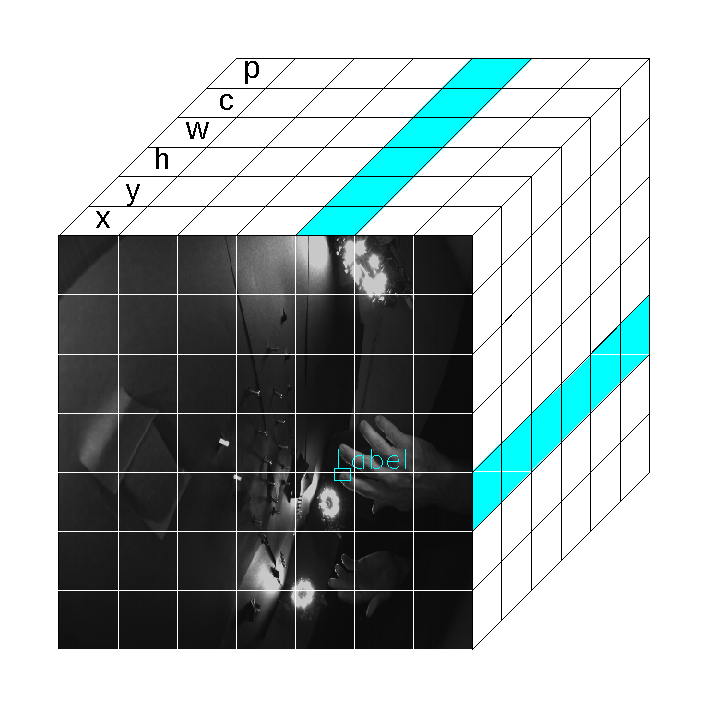
\includegraphics[width=.7\textwidth]{Kapitel/50Kostenfunktion/Bilder/PredictionTensor.pdf}
	\caption{Prediction-Tensor}
	\label{img:prediction_tensor}
\end{figure} 

Die Confidence war deshalb nicht explizit in den Labels enthalten, weil sie aus den Vorhersagen zu x, y, w und h sowie den entsprechenden Labels berechnet wurde.
Die Label-Confidence ist eigentlich nichts anderes als die IOU\footnote{\label{foot:1}IOU = Intersection Over Union} zwischen der vorhergesagten Bounding-Box und der Label-Bounding-Box einer bestimmten Gitterzelle. 
Die Berechnung der IOU aus diesen beiden Bounding-Boxen erfolgt wie aus Abbildung \ref{img:IOU} ersichtlich.

Es befinden sich allerdings in den meisten Gitterzellen keine rechten Zeigefinger. 
Aus diesem Grund existieren in diesen Gitterzellen auch keine Labels zu x,y,w und h, weshalb auch keine Label-Bounding-Boxen existieren.
In jeder dieser Gitterzellen, in welchen keine Label-Boundingboxen existieren ist die Label-Confidence automatisch=0. 
So wird man nach dem Training aufgrund der Confidence-Variable im Output für jede Gitterzelle ablesen können, ob sich darin irgend ein Objekt befindet, und wie gut dieses wahrscheinlich auf die Vorhersage von x,y,w und h passt.


%IOU
\begin{figure}	
	\centering
	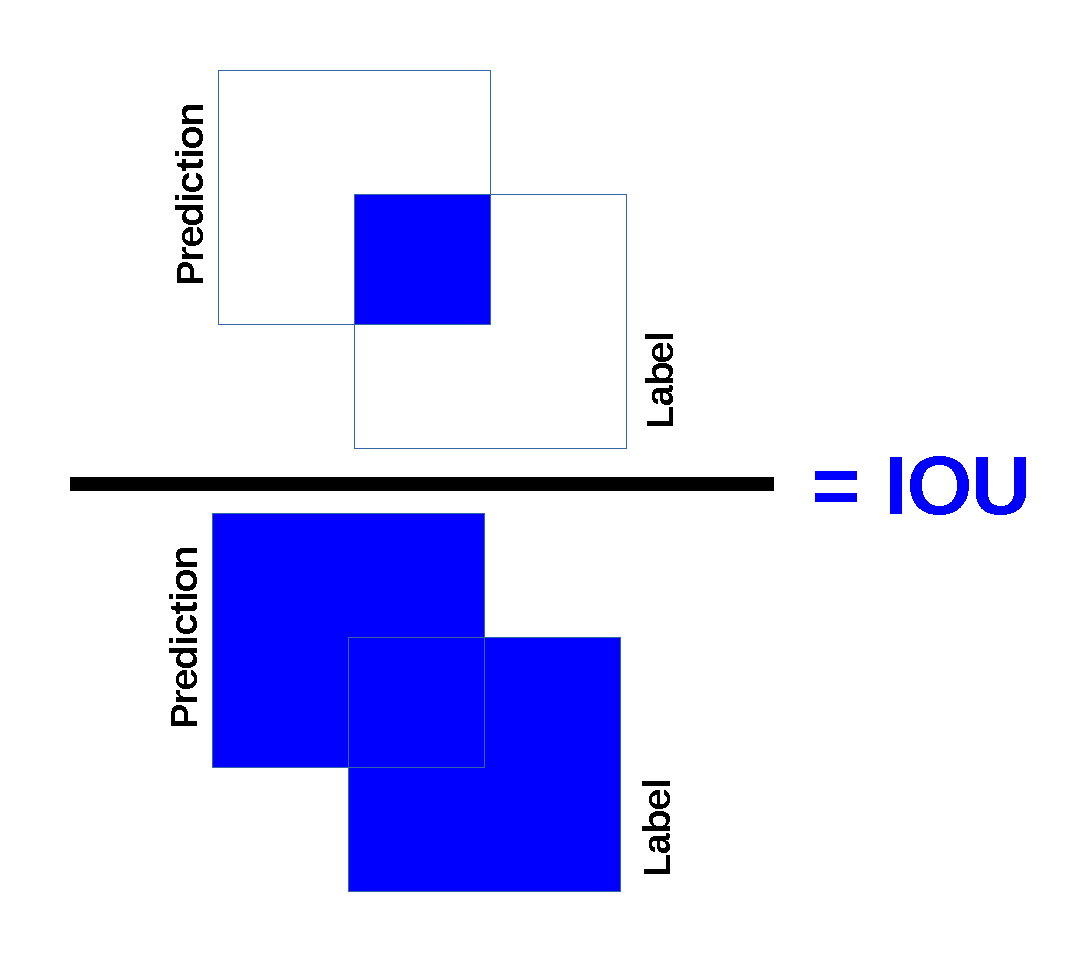
\includegraphics[width=.4\textwidth]{Kapitel/50Kostenfunktion/Bilder/IOU.pdf}
	\caption{Berechnung der IOU}
	\label{img:IOU}
\end{figure} 


\subsection{Design Kostenfunktion}
\label{chapter:design_kostenfunktion}

\begin{eqfloat}
\begin{equation}
\begin{split}
	\lambda_{coord} * \sum_{i}^{7*7}& \mathds{1}_{i}^{obj}[(x_{i}-\hat{x}_i)^{2} + (y_{i}-\hat{y}_i)^{2}] \\\
	+ \lambda_{coord} * \sum_{i}^{7*7}& \mathds{1}_{i}^{obj}[(\sqrt{w_{i}}-\sqrt{\hat{w}_{i}})^{2}+(\sqrt{h_{i}}-\sqrt{\hat{h}_{i}})^{2}] \\\
	+ \sum_{i}^{7*7}& \mathds{1}_{i}^{obj}[(C_{i} - \hat{C}_{i})^{2}] \\\
	+ \lambda_{noobj} * \sum_{i}^{7*7}& \mathds{1}_{i}^{noobj} [(C_{i} - \hat{C}_{i})^{2}] \\\
	+ \sum_{i}^{7*7}&\mathds{1}_{i}^{obj} (p_{i}-\hat{p}_{i})^{2}
\end{split} 
\end{equation}
\caption{abgespeckte Kostenfunktion wie Sie in dieser Arbeit verwendet wurde.}
\label{eq:Kostenfunktion}
\end{eqfloat}


\begin{table}
\centering
\begin{tabularx}{\textwidth}{|l|X|}
\hline  \textbf{Symbol} & \textbf{Definition}\\
\hline  $\lambda_{coord}$  & Faktor welcher verwendet wird um Fehler in den Koordinaten, sowie Höhe und Breite der Boundingboxen stärker zu gewichten. In diesem Fall wird hier ein Faktor von 5 verwendet. Diese Zahl ist so eins zu eins aus dem Yolo-Paper \cite{yolo} übernommen worden.\\
\hline  $\lambda_{noobj}$  & Faktor, welcher verwendet wird, damit der Confidence-Fehler nicht so stark gewichtet wird, wenn gar kein Objekt in dieser Gitterzelle vorhanden ist. In diesem Fall wird hier ein Faktor von 0.5 verwendet. Diese Zahl ist so eins zu eins aus dem Yolo-Paper \cite{yolo} übernommen worden.\\
\hline  $x_i$  & x-Labelkoordinaten, welche für die Gitterzelle i die Distanz vom Mittelpunkt der Boundingbox zum linken Rand der Gitterzelle i angibt.\\
\hline  $y_i$  & y-Labelkoordinaten, welche für die Gitterzelle i die Distanz vom Mittelpunkt der Boundingbox zum oberen Rand der Gitterzelle i angibt.\\
\hline  $w_i$  & Breite der Label-Boundingbox für die Gitterzelle i\\
\hline  $h_i$  & Höhe der Label-Boundingbox für die Gitterzelle i\\
\hline  $C_i$  & Label-Confidence für die Boundingbox in der Gitterzelle i\\
\hline  $p_i$  & Label-Wahrscheinlichkeit, dass sich ein rechter Zeigefinger in der Gitterzelle i befindet. \\	
\hline  $\hat{x},\hat{y},\hat{w},\hat{h},\hat{C},\hat{p}$  & Dies sind die Predictions des Netzwerks, welche den oben definierten entsprechenden Labels gegenübergestellt werden.\\
\hline  $\mathds{1}_{i}^{obj}$  & Dieses Objekt ist = 1, wenn in der Gitterzelle i ein rechter Zeigefingerspitz enthalten ist. Dieses Objekt ist = 0, wenn in der Gitterzelle i \textbf{kein} rechter Zeigefingerspitz enthalten ist.\\	
\hline  $\mathds{1}_{i}^{noobj}$  & Dieses Objekt ist = 1, wenn in der Gitterzelle i \textbf{kein} rechter Zeigefingerspitz enthalten ist. Dieses Objekt ist = 0, wenn in der Gitterzelle i ein rechter Zeigefingerspitz enthalten ist.\\
\hline $\sum_{i}^{7*7}$ & Summe über alle Gitterzellen, wobei i immer einer Gitterzelle entspricht.\\
\hline
\end{tabularx}
\caption{Beschreibung der Kostenfunktionselemente}
\label{tbl:beschr_kostenfuntion}
\end{table} 

Die Auswahl bzw. das Design der Kostenfunktion ist wahrscheinlich der wichtigste Schritt im Design eines Neuronalen Netzwerks. 
In dieser Arbeit bestand das grosse Glück, dass die Kostenfunktion grösstenteils vom Yolo v1-Paper \cite{yolo} vorgegeben wurde (Was auch mit ein Grund für die Wahl von Yolo v1 war).
Die Kostenfunktion, wie Sie in dieser Arbeit verwendet wurde kann man in Gleichung \ref{eq:Kostenfunktion} betrachten. 
Diese Kostenfunktion ist etwas einfacher als die Kostenfunktion, wie Sie im Yolo v1 Paper zu sehen ist. 
Dies hat zwei Gründe. 
Zum einen wurde pro Gitterzelle nur eine Boundingbox vorhergesagt. 
So fällt für Zeile 1-4 der Kostenfunktion das zweite Summenzeichen, sowie deren iteration über die Variable j weg. 
Zum anderen wurde nur eine Klasse(rechter Zeigefinger) gelabelt und vorhergesagt.
So fällt auf der Zeile 5 das Summenzeichen und deren entsprechende Iteration über alle Klassen weg.

Spannend war, dass es im aktuellen Fall für das Netzwerk nicht möglich war einen nach unten korrigierenden Einfluss auf die Variable $p_i$ zu nehmen.
So gingen die Vorhersagen für die $p_i$'s je länger man lernte desto stärker gegen 1.  
Der Grund dafür lag darin, dass $\mathds{1}_{i}^{obj}$ immer = 0 war, wenn \textbf{kein} rechter Zeigefingerspitz in dieser Gitterzelle enthalten ist.
So wird das Netzwerk nie korrigiert, wenn es die Wahrscheinlichkeit höher einschätzt, als sie tatsächlich ist. 
Dies stellte allerdings kein Problem dar. 
Denn die letztendliche Identifikation des Fingers, welche mit dem resultierenden Wert aus $c_i * p_i$ ermittelt wurde, war wegen der Nähe von $p_i$ zu 1 sozusagen gleichzusetzen mit $c_i$.
Da auch mit mehreren Klassen $c_i$ eine Dominante Rolle spielen würde, wenn es darum geht, ob ein Objekt erkannt wurde oder nicht, würde höchstwahrscheinlich die Performance nicht besser, wenn man Yolo mit mehr als einer Klasse trainieren würde.






 


\subsection{Fazit}
Folgende Punkte konnten aus dieser Arbeit gelernt werden, bzw. sollten im Falle einer Vertiefung beachtet werden. 
\begin{enumerate}
\item Man darf die Wahl der Kostenfunktion nicht unterschätzen. 
Wie man im Kapitel \ref{chapter:erster_wurf} sehen kann, darf man nicht annehmen, dass die Kostenfunktion frei und ohne gross nachzudenken gewählt werden kann. 
Vielmehr muss die Wahl der Kostenfunktion stark mit dem Netzwerk und dem Problem interagieren. 
\item Für die Zukunft zu beachten: In dieser Arbeit wurde pro Gitterzelle nur eine Boundingbox vorhergestagt (Dies weil die Komplexität von zwei Boundingboxen in Tensorflow nahezu jegliches Mass überstiegen hätte.). Wahrscheinlich könnte die Performance noch verbessert werden, wenn anstelle von einer min. zwei Boundingboxen pro Gitterzelle vorhergesagt würden. Dies aufgrund der Theorie \cite{PrivateCommunication}, dass mit mehreren Boundingboxen verschiedene Features eines Bildes verwendet werden können, um einen Finger vorherzusagen.
\todo[inline,size=\Large]{Dieses Fazit auf Redundanz prüfen}
\item Zum Vergleich: Im Paper Yolo v2 wurde anstelle von 7x7 Gitterzellen 13x13 Gitterzellen verwendet, was in einer höheren Präzision resultieren würde. 
Eine höhere Präzision wäre für das Endziel dieser Arbeit nur zu begrüssen. 
Wenn dies allerdings mit Yolo v1 umgesetzt würde, hätte man das Problem, dass wegen dem Grösseren Speicheraufwand, welcher für die zusätzlichen Elemente \grqq{}verbraucht\grqq{} würde die Minibatchsize verkleinert werden müsste. 
So wird angenommen, dass mit einer kompletten Umstellung auf Yolo v2 ein besseres Resultat erzielt würde, als wenn man Yolo v1 einfach erweitern würde.  
\end{enumerate}
